\documentclass[12pt,a4]{article}

\usepackage{inputenc}
\usepackage[T1]{fontenc}
\usepackage{amsmath,amsfonts,amsthm}
\usepackage{graphicx}

\newcommand{\R}{{\mathbb R}}
\newcommand{\C}{{\mathbb C}}
\newcommand{\N}{{\mathbb N}}
\newcommand{\ra}{\rightarrow}
\newcommand{\eps}{\varepsilon}
\newcommand{\cond}{\ensuremath{\text{cond}}}

\newtheorem{theorem}{Theorem}



\title{Inversion of the Laplace transform}
\author{Lasse Lybeck\\013748498}


\begin{document}

\maketitle

\section{Introduction}

Let $f:[0,\infty)\rightarrow \R$. The Laplace transform $F$ of $f$ is defined by
\begin{equation}\label{laplace}
 F(s) = \int_0^\infty e^{-st}f(t)dt,\quad s\in\C ,
\end{equation}
provided that the integral converges.

The transform has many applications in physical sciences and is therefore widely used and studied. One example of the usage of the transform is in linear differential equations, which may in some cases be easily solved using the Laplace transform.

The direct problem is to determine $F$ for a given function $f$ according to (\ref{laplace}). The inverse problem is: {\em given a Laplace transform $F$, find the corresponding function $f$.} In this study we will be looking at the inverse problem from the computational point of view. We will notice that the inverse problem is ill-posed and not at all trivial.




\section{Materials and Methods}\label{sec:methods}

\subsection{Theoretical basis}

In this study we will solve the inverse problem with the \emph{truncated singular value decomposition} method. In the future we will refer to the singular value decomposition as SVD. Let us first revise the theory for the SVD and the pseudoinverse.

\subsubsection{Singular value decomposition and the pseudoinverse}
\label{sec:svd}

The truncated SVD method is based on the fact that every matrix $A \in \R^{k \times n}$ can be decomposed into the product of three matrices
\begin{equation}
A = U D V^T,
\end{equation}
where $U$ and $V$ are orthogonal matrices and $D$ is a diagonal matrix. The diagonal elements $d_{i,i}$, $i = 1, \ldots , min \left\{ k,n \right\}$ of $D$ are called the \emph{singular values of $D$}.

The \emph{pseudoinverse} of $A$ (denoted as $A^+$) can be calculated via the SVD of $A$. We define the pseudoinverse of the diagonal matrix $D \in \R^{k \times n}$ as the diagonal matrix $D^+ \in \R^{n \times k}$ where the diagonal elements have the values
\begin{equation}
D^+_{i,i} =
\begin{cases}
    1 / d_{i,i} & \text{if }d_{i,i} \neq 0 \\
    0           & \text{otherwise}.
\end{cases}
\end{equation}
Now we can define the pseudoinverse of $A$ as 
\begin{equation}\label{pseudo}
A^+ = V D^+ U^T .
\end{equation}

It can be shown, that if $A$ is an invertible matrix, then $A^+ = A^{-1}$. This is however often not the case.

In the case of linear systems $Af = m$ we get the least squares solution easily with the pseudo inverse of $A$. As it is shown in \cite{samu}, theorem 4.1, the least squares solution to a system $Af = m$, where $A \in \R^{k \times n}$, is given by $A^+ m$. Notice that here $A$ need not be invertible, as it may not even be a square matrix.

\subsubsection{Truncated singular value decomposition}

Although we now know that linear systems of the type $Af = m$ can easily be solved with the pseudoinverse of the coefficient matrix $A$, this will not always be the proper way of solving inverse problems of the same type. Consider the following case.

Let $m = A f + \eps$, where $\eps$ is some small random noise. It would seem logical that this kind of a problem could be solved approximately with the same method as the problems described earlier with no noise present, as $Af + \eps \approx Af$. This will however not work, as we will come to see later. The reason to this comes from the so called \emph{condition number} of the coefficient matrix $A$.

The condition number of a matrix $A \in \R^{k \times n}$ is defined as the ratio of the largest and smallest singular of $A$. In the case $A$ has an SVD as described in section \ref{sec:svd}, the condition number is defined as $\cond(A) = d_1 / d_{min(k,n)}$.

In the case of ill-posed inverse problems the condition numbers are large and grow as the size of the matrix grows. This is the reason why naive inversion fails for these problems. As the condition number is large, the least singular values are correspondingly very small. This means that for the pseudoinverse $A^+$ the singular values are very large. As we try to calculate the least squares solution with the naive inversion the right side of the equation becomes $A^+ (Af + \eps)$, where we multiply $A^+$ with the noise $\eps$. This leads to a large error, even thou the noise is quite small, as the inverse singular values are often very much larger. This is the reason why naive inversion fails for ill-posed inverse problems.

The truncated SVD is a method that tries to solve this problem by "discarding" the singular values that are regarded as too small. For a \emph{regularization parameter} $\alpha > 0$, the truncated SVD for a matrix $A \in \R^{k \times n}$ in defined in the means of the SVD $A = U D V^T$ as $A_{\alpha} = U D_{\alpha} V^T$, where
\begin{equation}
(D_{\alpha})_{i,i} =
\begin{cases}
D_{i,i}, & \text{if } D_{i,i} \geq \alpha \\
0,       & \text{otherwise}.
\end{cases}
\end{equation}

Now the least singular value of $A_{\alpha}$ is no smaller that $\alpha$, and the problem with the naive inversion is solved, as long as the regularization parameter can be chosen well enough. We now have a reconstruction function
\begin{equation}
R_{\alpha}(m) = A_{\alpha}^+ m = V D_{\alpha} U^T m.
\end{equation}
This reconstruction model will be used in this study to solve the inverse Laplace transform. For further reading on truncated SVD, see \cite{samu}, chapter 4.1.



\subsection{The matrix model}\label{sec:matrixmodel}

Assume we know the values of $F$ at these real-valued points:
$$
 0<s_1<s_2<\ldots <s_n<\infty.
$$ 
Then we may approximate the integral in (\ref{laplace}) for example with the trapezoidal rule as
\begin{equation} \label{laptrap}
\begin{split}
 \int_0^\infty e^{-st}f(t)dt\, \approx\, \frac{t_k}{k} & \left( \frac{1}{2}e^{-st_1}f(t_1)+e^{-st_2}f(t_2)+e^{-st_3}f(t_3)+\ldots\right.\\   &\ \ \left. +e^{-st_{k-1}}f(t_{k-1})+\frac{1}{2}e^{-st_k}f(t_k)\right) ,
\end{split}
\end{equation}
where vector $t=[t_1\ t_2\ \ldots\ t_k]^T\in\R^k$, $0\leq t_1<t_2<\ldots <t_k$, contains the points at which the unknown function $f$ will be evaluated. By denoting $f_\ell=f(t_\ell), \ \ell=1,\ldots ,k$, and $m_j=F(s_j),\ j=1,\ldots ,n$, and using \eqref{laptrap}, we get a linear model of the form $m=Af+\epsilon$ with
\begin{equation}\label{LaplaceA} 
A = \frac{t_k}{k}\begin{bmatrix} \frac{1}{2}e^{-s_1t_1} & e^{-s_1t_2} & e^{-s_1t_3} & \ldots & e^{-s_1t_{k-1}} & \frac{1}{2}e^{-s_1t_k} \\
                       \frac{1}{2}e^{-s_2t_1} & e^{-s_2t_2} & e^{-s_2t_3} & \ldots & e^{-s_2t_{k-1}} & \frac{1}{2}e^{-s_2t_k} \\
                       \vdots & & & & & \vdots \\
                       \frac{1}{2}e^{-s_nt_1} & e^{-s_nt_2} & e^{-s_nt_3} & \ldots & e^{-s_nt_{k-1}} & \frac{1}{2}e^{-s_nt_k} \end{bmatrix}.
\end{equation}


\subsection{The inversion method}

As the materials for this study we have created MATLAB code for calculating the inverse Laplace transform with the truncated SVD method. The starting point for out experiments is as follows.

The measurements were done with the function $f: \left[ 0, \infty \right[ \ra \R$,
\begin{equation}\label{eq:f}
f(t) = 
\begin{cases}
1, & \text{for } 0 \leq t \leq 1 \\
0, & \text{otherwise}.
\end{cases}
\end{equation}

The matrix $A$ and vectors $s$ and $t$ are defined as explained in section \ref{sec:matrixmodel}. The values of $s_i$ of the vector $s \in \R^n$ and $t_j$ of the vector $t \in \R^k$ were chosen evenly spaced from the intervals $\left] 0, 100 \right[$ and $\left[ 0,3 \right]$, respectively. The values of $n$ and $k$ were varied in the experiments to determine their effect on the results.

With the specified function $f$ the Laplace transform can be calculated as
\begin{equation}
F(s) = \int_0^{\infty} e^{-st} f(t) dt
     = \int_0^1 e^{-st} dt
     = \frac{1 - e^{-s}}{s},
\end{equation}
and thus the values of the Laplace transform can be easily without using numerical integration methods. This adds both speed and precision to the calculations.

We then created the measurement points $m = [m_1, m_2, \ldots, m_n]^T + \eps$, where $m_i = F(s_i)$, $F$ is defined as in \eqref{laplace} for the function $f$ and $\eps$ is some random noise.

The reconstruction $T_\alpha(m)$ from the measurement data $m$ of the function $f$ in the interval $\left[0,3\right]$ could then be calculated with the truncated SVD method with $\alpha$ as the regularization parameter. The results were then recorded with different choices of $\alpha$.



\section{Results}\label{sec:results}

\begin{figure}[t]
\begin{center}
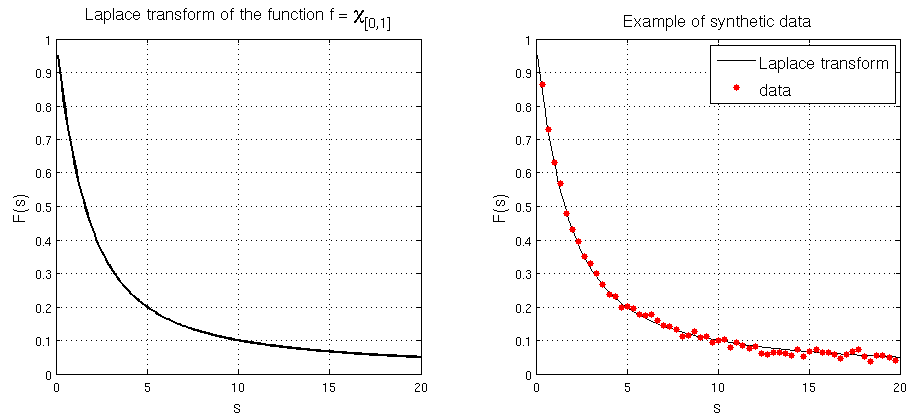
\includegraphics[scale=.5]{img/laplace_data.png}
\end{center}
\caption{Left: Laplace transform of $f$. Right: An example of synthetic data used in the experiments.}
\label{fig:laplace}
\end{figure}

\begin{figure}[t]
\begin{center}
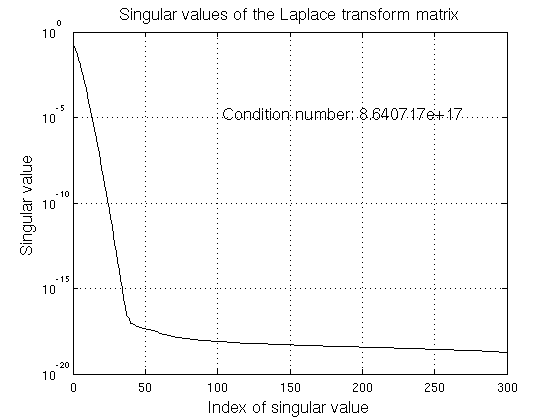
\includegraphics[scale=.4]{img/singular.png}
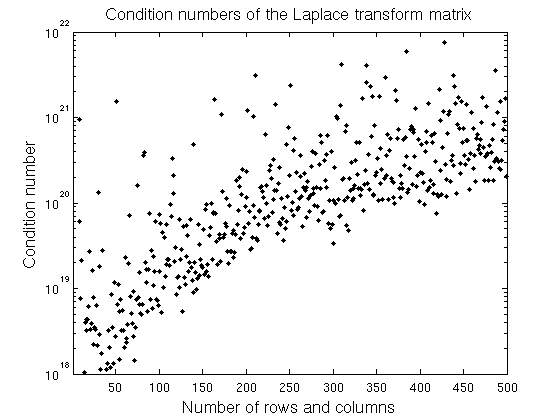
\includegraphics[scale=.4]{img/cond.png}
\end{center}
\caption{Left: Singular values of a Laplace transform matrix. Right: Condition numbers of $k \times k$ Laplace transform matrices}
\label{fig:singular}
\end{figure}

The Laplace transform of the function $f$ defined in \eqref{eq:f} is shown in figure \ref{fig:laplace}. An example of the synthetic measurement data used in the inversion of the Laplace transform can be seen in the right hand side plot in the same figure.

In the left hand side plot in figure \ref{fig:singular} the singular values are shown for a certain Laplace transform matrix $A$. The matrix is constructed with the vectors $t \in \R^k$ and $s \in \R^n$, with the values $k = 1000$ and $n = 300$. The condition number for the matrix is, as shown in the figure, $\cond(A) \approx 8.6407 \cdot 10^{17}$. In the right hand side plot is shown the condition number for a collection of square Laplace transform matrices. The side of the square matrices in the plot ranges from $1$ to $500$.





\section{Discussion}

\subsection{Ill-posedness}

As it can be seen from figure \ref{fig:singular}, the singular values of the coefficient matrix are decreasing very rapidly (notice the logarithmic scale on the y-axis). This results in high condition numbers and therefore in systems with high sensibility for noise. As it can further be seen from figure \ref{fig:cond}, the condition number greatly increases as the size of the matrix increases (again, notice the logarithmic scale). These results clearly point to the fact that the inverse Laplace transform is an ill-posed problem.


\newpage
\begin{thebibliography}{9}

\bibitem{samu}
Mueller, Jennifer L., ; Siltanen, Samuli \\
\emph{Linear and nonlinear inverse problems with practical applications} \\ Philadelphia : SIAM, 2012. - (Computational science \& engineering.)

\end{thebibliography}

\end{document}



